% =====================================================================
% DRAFT -- "Minkowski image loss and extreme events"
% Status (2026-09-17): introduction and methods drafted; Study 1 COMPLETE
% (six deterministic backbones) and Study 2 COMPLETE in-distribution
% (four flow-matching cells). Table~\ref{tab:iid} is populated from the
% 2026-09-17 evaluation sweep, every row at ONE peaks-over-threshold
% level, u = 31 mm/h. Table~\ref{tab:ood} remains a placeholder: the
% out-of-distribution protocol is not yet run.
% No results are fabricated: reported numbers are measured; all unrun
% cells are "--". All numbers are single-seed in training. Deterministic
% rows use the full test set (n = 285,383); the flow-matching rows of
% Table~\ref{tab:iid} a 4,096-patch subset (M = 16, 16 Heun steps) whose
% observed tail differs from the full set. Table~\ref{tab:prelim}'s
% flow-matching row and the dry-tail ratios predate that sweep (25,600
% patches, earlier protocol) and are TO BE REGENERATED.
% Table~\ref{tab:spread} measures how far each column moves between two
% draws of the same ensemble; nothing smaller than that is claimed.
% Source: eval_results/ at commit 63d0748 of
% github.com/fquaren/minkowski-loss.
% Citation identifiers: see header of references.bib for verification status.
% Scientific lower-casing applied throughout (flow matching, persistent
% homology, euler characteristic, etc.); eponyms capitalised (Pareto,
% Cauchy--Crofton, Gaussian, Reynolds).
% =====================================================================
\documentclass{article}
\usepackage{arxiv}
\usepackage[utf8]{inputenc} % allow utf-8 input
\usepackage[T1]{fontenc}    % use 8-bit T1 fonts
\usepackage{hyperref}       % hyperlinks
\usepackage{url}            % simple URL typesetting
\usepackage{booktabs}       % professional-quality tables
\usepackage{amsfonts}       % blackboard math symbols
\usepackage{amsmath}        % align, etc.
\usepackage{nicefrac}       % compact symbols for 1/2, etc.
\usepackage{microtype}      % microtypography
\usepackage{graphicx}
\usepackage{threeparttable}
\usepackage[numbers]{natbib}  % enables \citep/\citet
\graphicspath{ {./images/} {./figures/committee/} }

\title{Minkowski image loss and extreme events}

\author{
 Filippo Quarenghi \\
  FGSE\\
  University of Lausanne\\
  Lausanne, Switzerland\\
  \texttt{filippo.quarenghi@unil.ch} \\
   \And
 Ophelia Miralles \\
  AI Weather Research\\
  MetNorway\\
  Oslo, Norway\\
    \And
 Erwan Koch \\
  Expertise Center for Climate Extremes (ECCE)\\
  FGSE/HEC\\
  University of Lausanne\\
  Lausanne, Switzerland\\
  \And
 Tom Beucler \\
  FGSE\\
  University of Lausanne\\
  Lausanne, Switzerland\\
}

\begin{document}
\maketitle

\begin{abstract}
Statistical downscaling of precipitation must reproduce not only pointwise intensity
but the geometry of rain fields -- the size, boundary complexity, and connectivity of
wet regions -- and this requirement is most acute, and most poorly served by standard
pixelwise losses, in the extreme tail. We study whether the Minkowski image loss
\citep{quarenghi2026minkowski}, a structural loss built from differentiable surrogates
of the Minkowski functionals (area, perimeter, and a topological term) of precipitation
excursion sets, improves the super-resolution of \emph{extreme} precipitation when used
to train generative downscalers, and how it compares to other structural losses designed
for extremes. We pair an analytical, differentiable formulation of the functionals with a
residual flow-matching downscaler -- a deterministic backbone for the conditional mean and
a flow-matching model for the stochastic residual, following the corrective decomposition
of \citet{mardani2025corrdiff} -- and evaluate on EUMETNET OPERA radar precipitation at
$12.5\times$ super-resolution. The structural loss is coupled to the flow-matching model by
back-propagating its gradient through the last few steps of the probability-flow ordinary
differential equation. Crucially, we separate the loss comparison (deterministic backbones,
controlled) from the generative showcase (flow-matching models on a fixed reference
backbone), so that conclusions about the loss are not confounded by the generative stage
adapting to a weaker backbone. Extremes are evaluated with a tail-aware protocol combining
high-threshold Minkowski curves, peaks-over-threshold extreme-value statistics, and the
fractions skill score at high thresholds, under both in-distribution and
out-of-distribution extreme events.
On the deterministic backbone the loss buys a large tail gain for a small accuracy cost: the
fraction of observed heavy-rain exceedances the model reproduces rises from $0.12$ to $0.24$,
the mean absolute return-level bias falls from $0.64$ to $0.44$, and the fractions skill
score at $89\,\mathrm{mm\,h^{-1}}$ rises from $0.04$ to $0.16$, for $+3.8\,\%$ mean absolute
error. Four competing structural losses -- spectral, structural similarity, soft wet area,
and optical-flow consistency -- reproduce none of this: at weights that leave the mean
absolute error within $0.7\,\%$ of the baseline they leave the tail \emph{worse} than plain
mean squared error. On the generative stage the same loss, applied as a truncated-back-propagation
reward, produces a tail improvement that is at the edge of what the evaluation can resolve:
of seven columns, only the exceedance ratio and the spectral log-distance move by more than
two independent draws of the same ensemble move them. We trace this asymmetry to
a pixel-mass bottleneck: above $31\,\mathrm{mm\,h^{-1}}$ fewer than $10^{-4}$ of pixels
contribute, so the structural gradient is dominated by the drizzle thresholds regardless of
threshold weighting.
\end{abstract}

\keywords{statistical downscaling \and super-resolution \and extreme precipitation \and
flow matching \and structural loss \and Minkowski functionals \and persistent homology}

% =====================================================================
\section{Introduction}
% ---------------------------------------------------------------------
Super-resolution of precipitation fields is a central tool for bridging the gap between
coarse model or reanalysis output and the kilometre-scale information needed for impact
assessment. The task is hard precisely where it matters most: extreme rainfall is rare,
spatially intermittent, and heavy-tailed, so pointwise losses such as the mean squared
error both under-represent the tail and incur the double-penalty problem, in which a
spatially displaced but otherwise correct extreme is penalised twice. Minimising such
losses drives predictions toward the conditional mean, smoothing away the very gradients
and small-scale structures that characterise convective extremes.

Two complementary remedies motivate this work. First, \emph{structural} losses score the
geometry of the field rather than pixel-aligned intensity. The Minkowski image loss
\citep{quarenghi2026minkowski} is one such loss: it summarises each excursion set
$\{x \ge u\}$ of the field by its Minkowski functionals -- area $A$, perimeter $P$, and a
topological descriptor (the euler characteristic $\chi = \beta_0 - \beta_1$, or the
connected-component count $\beta_0$) -- and compares the resulting threshold curves
between prediction and target. By Hadwiger's theorem these three functionals form a
complete basis for motion-invariant, additive, continuous valuations in two dimensions,
and their rigid-motion invariance removes the spatial double penalty by construction.
Second, a learned data-manifold prior makes a low-dimensional structural loss safe to
apply: a purely deterministic generator trained against such a loss can \emph{game} it
(for instance, amplifying grid-aligned upsampling edges to manufacture ``free''
perimeter), whereas a generative model constrained to its data manifold cannot wander
off-manifold to exploit the reward. This motivates coupling the structural loss to a
generative downscaler rather than to a deterministic regressor alone.

The foundational study \citep{quarenghi2026minkowski} introduced the Minkowski image loss
and a learned emulator of the (non-differentiable) functionals, and documented two
findings we take as given here: the learned emulator is value-accurate but
derivative-wrong (a wrong-induced-metric pathology that yields poor input-space
gradients), and the deterministic-generator gaming failure mode above. In this paper we
ask a different, application-driven pair of questions, specific to extremes:
\begin{enumerate}
  \item Does training a generative super-resolution model with the Minkowski image loss
  improve the accuracy and the perceptual realism of \emph{extreme} precipitation fields,
  relative to the same model trained without it?
  \item How does the Minkowski image loss compare to other structural losses targeting
  extremes?
\end{enumerate}

Our contributions are: (i) an analytical, differentiable formulation of the Minkowski
functionals with threshold-localised gradients, including a connected-component variant
via differentiable persistent homology for hole-rich fields; (ii) a residual flow-matching
downscaler coupled to this loss by truncated back-propagation through the probability-flow
ordinary differential equation; (iii) a
controlled two-study experimental design that disentangles the effect of the loss from
the effect of the generative stage; and (iv) a tail-aware evaluation protocol for extreme
precipitation combining high-threshold Minkowski curves, peaks-over-threshold
extreme-value statistics, and the fractions skill score, applied to both in-distribution
and out-of-distribution extremes.

% =====================================================================
\section{Related work}
% ---------------------------------------------------------------------
\paragraph{Generative downscaling.} Diffusion and flow-based models dominate stochastic
precipitation super-resolution. We adopt \emph{flow matching} as the generative mechanism
\citep{lipman2023flowmatching, liu2023rectifiedflow}, a special case of the
stochastic-interpolant family \citep{albergo2023stochastic} that learns a velocity field
transporting a base density to the data and samples by integrating the probability-flow
ordinary differential equation. We combine it with the corrective (residual) decomposition
of \citet{mardani2025corrdiff}, in which a deterministic network predicts the conditional
mean and the generative model learns only the residual, isolating the stochastic,
fine-scale content in a manner analogous to Reynolds decomposition. A conditional denoising
diffusion model serves as a generative baseline. A recent intercomparison of generative
precipitation downscalers \citep{wardleikis2025intercomparison} finds that residual diffusion
models reproduce fine-scale spatial structure well, but that intensity constraints -- readily
imposed on adversarial losses -- are non-trivial to incorporate into the noise-prediction
objective of diffusion models, leaving physical constraints on such models an open problem. The
same difficulty applies to the velocity-prediction objective of flow matching; evaluating the
structural loss on the clean-field estimate $\hat{x}_1$ rather than on the velocity target is our
route around it.

\paragraph{Structural and topological descriptors.} The Minkowski functionals and the
integral-geometric (Cauchy--Crofton) estimators we use are classical objects of
stochastic and integral geometry \citep{schneider2008stochastic}; the topological term is
grounded in computational topology and persistent homology
\citep{edelsbrunner2010computational}. Where the connected-component count is required, we
use the differentiability of persistence-based functions
\citep{carriere2021optimizing}.

\paragraph{Statistics-constrained learning for extremes.} Closest in spirit to this work is
extreme-event-aware ($\eta$-) learning \citep{chang2026eta}, which regularises training by
enforcing the statistics of a scalar observable indicative of extremeness, and proves
optimal-transport bounds showing that this controls the tail error of the learnt model even
when the training data contain no extremes. Our area channel is an instance of the same
mechanism -- matching a survival function is matching a $1$-Wasserstein distance
(Section~\ref{sec:theory}) -- with a vector-valued observable in place of a scalar one, which
is the extension their paper names as future work. The perimeter and topology channels go
beyond that framework: they constrain the geometry of the excursion set at a given level
rather than its measure, and carry no corresponding transport guarantee.

\paragraph{Coupling structural losses to generative models.} Using a differentiable
functional of generated samples as a training reward connects to reward fine-tuning of
diffusion and flow models \citep{clark2024draft}, whose documented failure modes (reward
hacking, diversity collapse) directly inform the guardrails we adopt.

\paragraph{Extreme-precipitation evaluation.} For tail-focused assessment we use
extreme-value theory in its peaks-over-threshold form \citep{coles2001} and the
fractions skill score \citep{roberts2008fss}, a scale-aware neighbourhood score that
mitigates the double-penalty problem and is evaluated per intensity threshold.

% =====================================================================
\section{Methods}
% ---------------------------------------------------------------------

\subsection{Problem setup and data}
We consider $12.5\times$ super-resolution of EUMETNET OPERA radar precipitation to a
$2\,\mathrm{km}$ grid, on $128\times128$ patches (pixel area $a_{\mathrm{px}} =
4\,\mathrm{km}^2$). Networks operate in a log-normalised space; all Minkowski functionals
and their offline targets are computed in physical units ($\mathrm{mm\,h^{-1}}$), with a
differentiable map from the network output back to physical intensity so that gradients
propagate to the model. The drizzle threshold is $0.1\,\mathrm{mm\,h^{-1}}$.

\subsection{The Minkowski image loss}
\label{sec:loss}
For a field $x$ and a set of intensity thresholds $u^{(1)} < \dots < u^{(Q)}$, each
excursion set $\{x \ge u^{(i)}\}$ is summarised by area $A(u)$, perimeter $P(u)$, and a
topological term $T(u)$, stacked over thresholds into a $\gamma$-vector
$\gamma = [A, P, T]$. The loss is the $L_1$ distance between log-transformed prediction and
target $\gamma$-curves, integrated over the log-intensity axis $\xi = \log u$,
\begin{equation}
  \mathcal{M}(\hat{\gamma}, \gamma)
  = \sum_{c \in \{A,P,T\}} \frac{1}{\xi_Q - \xi_1} \int_{\xi_1}^{\xi_Q}
    \bigl| \log \hat{\gamma}_c(e^{\xi}) - \log \gamma_c(e^{\xi}) \bigr| \, \mathrm{d}\xi ,
\end{equation}
with $\log 1p$ for the non-negative channels and a signed log for $\chi$, and the thresholds
placed log-uniformly over a fixed physical range, $0.1$ to $150\,\mathrm{mm\,h^{-1}}$ in $15$
levels.

The measure matters as much as the grid, and the two must be changed together. An earlier
version indexed the thresholds by climatological quantile and integrated $\mathrm{d}q$; there,
extending the grid into the tail is futile, because a threshold in $[0.999, 0.9999]$ carries
weight $10^{-4}$ however far the grid is extended. Integrating $\mathrm{d}\xi$ over fixed
physical levels instead gives each \emph{decade of intensity} equal weight: the deepest
threshold's weight rises by a factor of about $400$ relative to the quantile measure, and the
weights are near-uniform across levels. Fixed physical levels also remain comparable across
datasets and can be aligned with the evaluation thresholds. Because the numerical value of
$\mathcal{M}$ depends on this choice, values computed on the quantile grid and on the
log-physical grid are not comparable, and the $\gamma$ targets must be regenerated whenever
the grid changes.

\subsection{What the functionals estimate for extremes}
\label{sec:theory}
Beyond the completeness argument, each functional has an individual, tail-relevant
interpretation that motivates its use for extremes; each also carries a distinct assumption
footprint, which we state explicitly.

\paragraph{Area is the marginal survival function.} By definition
$A(u) = \int_D \mathbf{1}[X(s) \ge u]\,\mathrm{d}s$, so for a marginally stationary field
$\mathbb{E}[A(u)] = |D|\,\bigl(1 - F_X(u)\bigr)$: the area curve is the marginal survival
function scaled by domain area. Matching $A(u)$ on a grid that reaches into the tail
therefore matches the exceedance probabilities that a peaks-over-threshold analysis
summarises by a generalised Pareto shape and scale \citep{coles2001}. This link needs only
marginal stationarity -- no Gaussianity, no smoothness -- and so applies directly to
precipitation. It is also the channel a pointwise mean-squared-error most clearly neglects:
minimising the mean squared error targets the conditional mean, not the survival function,
and thus systematically under-populates high thresholds.

This makes the area channel an optimal-transport distance, not merely a correlate of one.
For non-negative variables the $L_1$ distance between survival functions is exactly the
$1$-Wasserstein distance between the corresponding laws,
$\int_0^\infty |S_1(u) - S_2(u)|\,\mathrm{d}u = W_1(F_1, F_2)$, so
\begin{equation}
  \int_0^\infty \bigl| \mathbb{E}[\hat{A}(u)] - \mathbb{E}[A(u)] \bigr| \,\mathrm{d}u
  = |D| \; W_1\!\left(F_{\hat{X}}, F_X\right) .
  \label{eq:w1}
\end{equation}
Matching expected areas across a threshold grid is therefore a discretised, reweighted
estimate of $W_1$ between the predicted and observed marginal intensity laws. This connects
the area channel directly to the optimal-transport framework of $\eta$-learning
\citep{chang2026eta}, in which enforcing the statistics of a scalar observable of
extremeness during training is shown to control the Wasserstein error of the learnt model in
the tail. Two differences of substance remain. Their observable is scalar and ours is a
three-component curve over thresholds, which is their stated direction for future work; and
our implementation integrates $|\log \hat{A} - \log A|\,\mathrm{d}\xi$ rather than
$|\hat{A} - A|\,\mathrm{d}u$, so equation~\eqref{eq:w1} holds for the unweighted, unlogged
form and our loss is a reweighting of it that trades exactness for near-uniform weight across
decades of intensity. The perimeter and topology channels have no such identity and are not
optimal-transport distances at all.

\paragraph{The topological term tracks the spatial maximum.} For a smooth, stationary
Gaussian (or Gaussian-related) field, the expected-Euler-characteristic heuristic states that
$\mathbb{P}\bigl(\sup_D X \ge u\bigr) = \mathbb{E}\bigl[\chi(A_u)\bigr]$ up to an error that
is super-exponentially small as $u \to \infty$ \citep{taylor2005validity, adler2007random}.
At high thresholds the excursion set loses its holes, so $\chi(A_u) \to \beta_0(A_u)$, the
count of distinct exceedance cells, and $\mathbb{E}[\beta_0(A_u)] \approx
\mathbb{P}(\sup_D X \ge u)$ -- precisely the block-maximum quantity of spatial
extreme-value theory. The topological channel at high $u$ is thus an estimator of the
field-maximum exceedance probability, the most extreme-relevant scalar the loss contains,
and this is the theoretical reason to prefer the connected-component count $\beta_0$ over
$\chi$ for extremes. The caveat is that this identity is proven for smooth Gaussian fields,
whereas precipitation is non-negative, intermittent, heavy-tailed and non-smooth; for our
data it is therefore a motivating heuristic rather than a theorem, and the
$\beta_0$--maximum correspondence is one we test empirically rather than assume.

\paragraph{Perimeter constrains the sharpness of extremes.} By the Kac--Rice / coarea
identity, the expected perimeter at level $u$ is $\mathbb{E}[P(u)] = \int_D
\mathbb{E}\bigl[\,\lVert \nabla X(s) \rVert \mid X(s) = u\,\bigr]\,p_X(u)\,\mathrm{d}s$
\citep{adler2007random}, the conditional mean gradient magnitude at the crossing level
weighted by the level density. Two fields with identical area at a high threshold -- the
same fraction of extreme rain -- but different perimeter differ in spatial concentration: a
diffuse plateau versus a compact convective cell. Perimeter thus encodes a property of
extremes that pointwise losses cannot distinguish, the steepness and cellularity of the
heaviest rain.

\paragraph{Consequences and limits.} Two consequences shape the method. First, all three
interpretations are tail-relevant \emph{only where the thresholds lie and only where the
excursion sets are non-empty}. A climatological quantile grid saturating in the moderate-rain
regime constrains bulk geometry and never samples the tail, which is why we replaced it with
fixed log-spaced physical levels reaching $150\,\mathrm{mm\,h^{-1}}$. That change is
necessary but, as Section~\ref{sec:results} shows, not sufficient: a threshold whose
excursion set is empty in almost every training sample contributes no gradient no matter what
weight the measure assigns it, and above $31\,\mathrm{mm\,h^{-1}}$ that is the operative
regime. The reach of the loss into the tail is therefore set by the exceedance rate in a
training batch, not by the threshold grid. Second, matching functional curves is necessary
but not sufficient: Hadwiger
completeness concerns the basis of valuations, not identifiability of the field law, and in
particular the functionals are marginal and cell-count descriptors that say nothing about
spatial \emph{tail dependence} -- whether distant extremes co-occur -- which is central to
spatial extreme-value theory and on which two fields with identical Minkowski curves may
differ. The loss therefore targets the marginal tail, the field-maximum law, and extreme
sharpness, but not the full extremal dependence structure.

\subsection{Analytical differentiable functionals}
\label{sec:analytical}
We compute the functionals analytically and differentiably, rather than emulating them.
Soft excursion sets use a sigmoid indicator $s^{(i)} = \sigma\!\big((x - u^{(i)})/\tau\big)$
with a proportional, annealed temperature $\tau$, so that gradients are supported on the
near-threshold band.

\paragraph{Area.} A straight-through estimator returns the exact discrete count in the
forward pass while back-propagating the soft gradient: with $\text{hard} = \mathbf{1}[x \ge u]$
and $s_{\mathrm{area}} = \text{hard} + (s - \mathrm{sg}[s])$ (where $\mathrm{sg}$ is
stop-gradient), the reported area is the unbiased $a_{\mathrm{px}} \sum \mathbf{1}[x\ge u]$
and the gradient is $\partial A/\partial x_j = a_{\mathrm{px}}\,\sigma'/\tau$
\citep{bengio2013ste}. This removes the soft-area bias while keeping a localised gradient.

\paragraph{Perimeter.} We use the isotropic Cauchy--Crofton estimator, a weighted count of
boundary crossings along axial and diagonal directions, which is rotation-invariant and
unbiased to within $\sim2\%$ of the continuous perimeter; the marching-squares alternative
overestimates curved boundaries and the central-difference total variation is anisotropic
and vanishes on one-pixel filaments. The offline target uses the identical estimator and
weights, so the loss minimum is unbiased.

\paragraph{Topology.} Two modes are provided. The euler characteristic
$\chi = V - E + F$ is computed locally on the cubical complex with a G\"odel (min) t-norm;
its hard limit is the 4-connected euler number. The connected-component count $\beta_0$ is
computed by differentiable persistent homology: dim-0 superlevel-set persistence yields
birth/death pairs whose critical pixels carry the gradient \citep{carriere2021optimizing},
and a soft, persistence-gated count reproduces the offline target. The two are not
interchangeable: $\chi = \beta_0 - \beta_1$ is dominated by the hole count $\beta_1$ in
hole-rich precipitation fields, so for connectivity-focused objectives $\beta_0$ is the
appropriate target and $\chi$ should not be substituted for it. The relative suitability of
$\chi$ versus $\beta_0$ for precipitation is examined empirically (Section~\ref{sec:disc}).

\subsection{Flow-matching downscaling and coupling}
We use conditional \emph{flow matching} as the generative stage. With $x_1$ the
high-resolution target, $x_0$ a base-noise sample, and $c$ the conditioning (upsampled
low-resolution precipitation concatenated with normalised orography), the linear-interpolant
path is $x_t = (1-t)\,x_0 + t\,x_1$ with target velocity $u = x_1 - x_0$, and a network
$v_\theta(x_t, t, c)$ is trained to regress $u$ under a mean-squared error
\citep{lipman2023flowmatching, liu2023rectifiedflow, albergo2023stochastic}. The base density
$x_0 \sim p_0$ is standard Gaussian by default; because precipitation residuals are heavy-tailed,
we optionally replace it with a unit-variance Student-t prior with $\nu$ degrees of freedom
(recovering the Gaussian as $\nu \to \infty$), a change shown to improve rare-event capture in
diffusion and flow models at negligible implementation cost \citep{pandey2025heavytailed}; we
treat $\nu$ as an ablation. Following the
corrective decomposition \citep{mardani2025corrdiff}, a deterministic backbone first
predicts the conditional mean $\mu(c)$ and the flow-matching model learns only the residual
$r = x_1 - \mu(c)$. Samples are drawn by integrating the probability-flow ordinary
differential equation over $t \in [0,1]$ with a small number of Euler or Heun steps. The
Minkowski functionals are evaluated on the clean-field estimate
$\hat{x}_1 = x_t + (1-t)\,v_\theta(x_t, t, c)$ (with $\mu(c)$ added back), never on an
intermediate state $x_t$. Flow matching has been reported to underestimate the upper
precipitation tail; we measure this dry-tail bias on the clean (pre-coupling) model as a
baseline. The deficit is present and grows with quantile: on the patches that contain
extremes the generated-to-target intensity ratio is $0.86$ at $q=0.99$ and $0.72$ at
$q=0.999$, against $0.94$ and $0.88$ over all patches. The tail under-estimation is
therefore concentrated exactly where the reward is meant to act, and it is accompanied by an
excursion-set discrepancy of the same sign -- the median ratio of predicted to observed patch
maximum is $0.81$ (Section~\ref{sec:results}).%
% [CITATION TO VERIFY: flow-matching dry-tail-bias preprint from the project notes; add once confirmed.]

\paragraph{Per-sample versus distributional reward.} The reward can be applied per sample --
penalising each generated field against a single target $\gamma$-curve -- or
distributionally, matching the \emph{distribution} of generated functionals to that of the
targets across an ensemble drawn from the same condition. The tail interpretations of
Section~\ref{sec:theory} favour the distributional form. The extreme-relevant quantities are
ensemble expectations: $\mathbb{E}[A(u)]$ is the survival function and
$\mathbb{E}[\beta_0(A_u)]$ the field-maximum exceedance probability, neither of which is a
property of any single draw. A per-sample structural reward, moreover, has no unique target
for a stochastic residual -- many distinct extreme fields are consistent with one coarse
condition -- and pushing every draw toward one structurally correct curve risks the
diversity collapse documented for reward fine-tuning \citep{clark2024draft}, destroying the
very spread that encodes the maximum law. Matching the distribution of $\gamma$ across the
ensemble is therefore the target aligned with the extreme-value quantities.

We implement the distributional form as an energy score on the $\gamma$-curves. Write
\begin{equation}
  D(a, b) = \sum_{c \in \{A,P,T\}} \frac{1}{\xi_Q - \xi_1}
  \int_{\xi_1}^{\xi_Q} \bigl| \log a_c(e^{\xi}) - \log b_c(e^{\xi}) \bigr| \,\mathrm{d}\xi
\end{equation}
for the threshold-integrated distance between two log-$\gamma$ curves, which is the loss
$\mathcal{M}$ of Section~\ref{sec:loss} evaluated on a pair of curves. For an ensemble
$\hat{\gamma}^{(1)}, \dots, \hat{\gamma}^{(M)}$ generated from one condition and the target
$\gamma$, the reward is
\begin{equation}
  \mathcal{E}\bigl(\{\hat{\gamma}^{(m)}\}, \gamma\bigr)
  = \frac{1}{M} \sum_{m=1}^{M} D\bigl(\hat{\gamma}^{(m)}, \gamma\bigr)
  \;-\; \frac{1}{2M(M-1)} \sum_{m \neq m'} D\bigl(\hat{\gamma}^{(m)}, \hat{\gamma}^{(m')}\bigr) .
  \label{eq:energy}
\end{equation}
The first term pulls the ensemble toward the target and the second pushes its members apart;
the balance is what makes the score proper, so that $\mathcal{E}$ is minimised at the true
ensemble dispersion rather than at zero spread, which is where the per-sample reward
$M^{-1}\sum_m D(\hat{\gamma}^{(m)}, \gamma)$ places its minimum. We verified this numerically
on synthetic ensembles of known dispersion. Two implementation points carry the guarantee. The
second term is normalised by $M(M-1)$ rather than $M^2$: the $M^2$ version is biased and its
minimiser sits at too little spread. And propriety holds because $D$ is an $L_1$ distance and
therefore of negative type; substituting a discrepancy that is not, such as a squared
difference of curves, forfeits it.

The distributional form is more costly -- an ensemble is required per gradient step, on top of
the truncated-ODE back-propagation -- so we treat the per-sample versus distributional choice
as an experimental factor rather than fixing it a priori.

To couple the structural loss, the pretrained flow-matching model is kept clean and a frozen
copy is retained as a reference. The Minkowski reward gradient is back-propagated through
only the last $K$ integration steps (truncated back-propagation through the ordinary
differential equation solver), which is memory-tractable and conveniently restricts the
structural signal to the low-noise, late-$t$ regime where $\hat{x}_1$ is sharp and the
functionals are meaningful \citep{clark2024draft}; we fine-tune low-rank adapters with
gradient checkpointing rather than the full model. Reward hacking and diversity collapse are
guarded against by (i) a proximal anchor to the frozen reference, (ii) the dense,
multi-threshold $\gamma$-reward matched distributionally across an ensemble (above), and
(iii) early stopping on a held-out structural metric the reward does not directly optimise,
such as the fractions skill score or an isoperimetric-violation rate.

\subsection{Competing structural losses}
\label{sec:competing}
Study~1 (Section~\ref{sec:design}) compares the Minkowski loss against four structural losses
built on different geometric or perceptual principles. All four are auxiliary terms added to
the pixelwise mean squared error, $\mathcal{L} = \mathcal{L}_{\mathrm{mse}} + w\,\mathcal{L}_{\mathrm{aux}}$,
with $w$ chosen independently for each loss and not comparable across losses.

\paragraph{Spectral kernel-CRPS.} A sample-based energy-score loss on the two-dimensional
Fourier magnitude. Let $\Phi(x) = |\widehat{x}|$ denote the magnitude of the two-dimensional
real FFT of field $x$, flattened to a vector. For a predicted ensemble
$\{\hat{x}^{(1)}, \dots, \hat{x}^{(M)}\}$ and target $x$,
\begin{equation}
  \mathcal{L}_{\mathrm{spec}}
  = \frac{1}{M}\sum_{m=1}^{M} \bigl\| \Phi(\hat{x}^{(m)}) - \Phi(x) \bigr\|_1
  - \frac{1}{2M^2}\sum_{m,m'=1}^{M} \bigl\| \Phi(\hat{x}^{(m)}) - \Phi(\hat{x}^{(m')}) \bigr\|_1 ,
\end{equation}
with the $\ell_1$ norms taken as means over frequency bins. For the deterministic backbones of
Study~1, $M = 1$ and the second term vanishes, leaving the first term alone -- an $L_1$
distance between Fourier magnitudes, not an energy score. This is a spectral analogue of
$\mathcal{M}$'s area channel restricted to Fourier space, but with no threshold structure and
no tail weighting: every frequency contributes equally regardless of the intensities that
produce it.

\paragraph{Structural similarity.} The single-scale SSIM loss, computed locally with an
$11\times11$ uniform window (mean $\mu$, variance $\sigma^2$, covariance $\sigma_{xy}$, data
range $R$ estimated per patch from $\max - \min$ over predicted and target values):
\begin{equation}
  \mathcal{L}_{\mathrm{ssim}}
  = \Bigl\langle \max\Bigl(0,\; \tfrac{1}{2}\Bigl(1 - \frac{(2\mu_{\hat{x}}\mu_x + c_1)(2\sigma_{\hat{x}x} + c_2)}
    {(\mu_{\hat{x}}^2 + \mu_x^2 + c_1)(\sigma_{\hat{x}}^2 + \sigma_x^2 + c_2)}\Bigr)\Bigr) \Bigr\rangle ,
  \qquad c_i = (k_i R)^2 ,
\end{equation}
with $k_1 = 0.01$, $k_2 = 0.03$, and $\langle\cdot\rangle$ the mean over pixels and windows.
This penalises local luminance, contrast, and correlation mismatch at a fixed spatial scale;
it has no notion of threshold or intensity level and treats a mismatch at $1\,\mathrm{mm\,h^{-1}}$
the same as one at $100\,\mathrm{mm\,h^{-1}}$ if the local contrast and correlation structure
are equally disturbed.

\paragraph{Soft wet-area.} A differentiable, weighted mismatch of the wet/dry mask at one
fixed threshold, using $u_0 = 0.1\,\mathrm{mm\,h^{-1}}$ (the drizzle threshold) and temperature
$\tau = 0.05$ (an earlier default of $\tau = 0.1$ at $u_0 = 0$ scored a dry pixel as $0.5$ wet
and was corrected):
\begin{equation}
  m(x) = \sigma\!\left(\frac{x - u_0}{\tau}\right)
\end{equation}
\begin{equation}
  \mathcal{L}_{\mathrm{wet}} = \Bigl\langle
    w_{\mathrm{fp}}\,\bigl[\mathrm{relu}(m(\hat{x}) - m(x))\bigr]^2
    + w_{\mathrm{fn}}\,\bigl[\mathrm{relu}(m(x) - m(\hat{x}))\bigr]^2 \Bigr\rangle
\end{equation}
with $w_{\mathrm{fp}} = w_{\mathrm{fn}} = 1$. This is the area channel of $\mathcal{M}$ evaluated
at a single threshold rather than a log-spaced grid, with a squared rather than logarithmic
penalty, and with no perimeter or topological term: it constrains how much area is wet, not
its shape, and only at the drizzle level.

\paragraph{Optical-flow consistency.} A motion-compensated teacher-student loss. A dense flow
field $(f_x, f_y)$ is estimated between the conditioning (low-resolution) precipitation field
$c$ and the target $x$ by block matching -- for each working-resolution pixel, the displacement
minimising the local sum of squared differences over a patch of size $21$, searched over a
radius of $4$ pixels -- then the conditioning field is advected by that flow to produce a
teacher field $\tilde{c} = \mathrm{warp}(c, f_x, f_y)$. The loss is a masked Huber distance
between the prediction and the teacher,
\begin{equation}
  \mathcal{L}_{\mathrm{flow}} = \Bigl\langle
    \mathbb{1}\bigl[\tilde{c} > \tau_m \;\lor\; x > \tau_m\bigr] \cdot
    H_\delta\bigl(\hat{x} - \tilde{c}\bigr) \Bigr\rangle , \qquad
  H_\delta(r) = \begin{cases} \tfrac{1}{2}r^2 & |r| \le \delta \\
    \delta\bigl(|r| - \tfrac{1}{2}\delta\bigr) & |r| > \delta \end{cases}
\end{equation}
with mask threshold $\tau_m = 0.05\,\mathrm{mm\,h^{-1}}$ and $\delta = 0.2$. This penalises
deviation from a motion-extrapolated baseline rather than from the true target directly, and
it constrains local advection consistency rather than the excursion-set geometry at any
intensity level.

\paragraph{What distinguishes the Minkowski loss from all four.} None of the four alternatives
has a threshold grid reaching into the tail with uniform weight in log-intensity. The spectral
and SSIM losses have no threshold at all; the soft wet-area loss has exactly one, fixed at
drizzle; the optical-flow loss has none and instead constrains motion. Only $\mathcal{M}$
(Section~\ref{sec:loss}) is built so that a term explicitly targets $89\,\mathrm{mm\,h^{-1}}$
and above with the same nominal weight as a term at $1\,\mathrm{mm\,h^{-1}}$. Section~\ref{sec:results}
shows that this structural difference, not merely a difference in overall loss magnitude,
tracks the difference in outcome: all four alternatives improve the tail less than plain mean
squared error at a weight that leaves point accuracy unchanged, while the Minkowski loss
improves it substantially at a comparable point-accuracy cost to what these losses pay for
no tail gain.

\subsection{Extreme-event evaluation protocol}
\label{sec:eval}
Standard wet-pixel-quantile thresholds saturate well below extreme intensities and spend
most of their resolution on light rain; for extremes we therefore extend the threshold
grid into the upper tail (e.g.\ $q \ge 0.999$ or fixed heavy-rain levels) and condition the
evaluation on patches that actually contain extremes (e.g.\ the top percentile by patch
maximum), since most patches contain none. Tail accuracy is assessed by (i) high-threshold
Minkowski curves; (ii) a peaks-over-threshold treatment fitting a generalised Pareto
distribution to exceedances and comparing tail shape, scale, and return levels
\citep{coles2001}; and (iii) the fractions skill score at high thresholds
\citep{roberts2008fss}. We evaluate both in-distribution and out-of-distribution extremes;
the latter are characterised by data analysis and held out from training. As a diagnostic
of emulator reliability, we plot the residual $\hat{\gamma} - \gamma$ against intensity on
test-set extremes: a mean-zero, symmetric residual supports an uncertainty estimate via the
trust parameter $\tau$, whereas a systematic (e.g.\ underestimation) bias indicates that
$\tau$ alone is insufficient and that augmentation with generated extremes is needed.

\paragraph{Choice of the peaks-over-threshold level.} We fit all generalised-Pareto
quantities at a single level, $u = 31\,\mathrm{mm\,h^{-1}}$. This level is chosen for
estimability, not because it delimits a physically meaningful class of event: it leaves
$316{,}652$ exceedances on the test set, enough for a stable shape estimate, whereas
$u = 53\,\mathrm{mm\,h^{-1}}$ leaves $112{,}471$ and drives the fitted observed shape from
$\hat{\xi} = +0.176$ to $-0.190$ -- a sign change, and therefore a change in whether the
fitted tail has a finite upper endpoint at all. Two consequences follow. First, every row of
a table must be fitted at the same $u$: the shape error and the return-level bias are
measured against an \emph{observed} fit that depends on $u$, so rows at different levels are
not comparable, and mixing them is the single most common way this comparison goes wrong.
Second, $u = 31\,\mathrm{mm\,h^{-1}}$ sits well below the extreme regime the paper is about
(the top-percentile patch maximum is $\approx 123\,\mathrm{mm\,h^{-1}}$), so the
peaks-over-threshold columns describe the upper-moderate tail, and the genuinely extreme
behaviour is read from the return levels extrapolated from that fit and from the fractions
skill score at $89\,\mathrm{mm\,h^{-1}}$.

\paragraph{Which tail columns carry weight.} We report the exceedance-count ratio
(predicted over observed number of exceedances of $u$) and the mean absolute relative
return-level bias as the primary tail columns, and we demote the generalised-Pareto shape
error $|\hat{\xi}_{\mathrm{pred}} - \hat{\xi}_{\mathrm{obs}}|$ to a secondary diagnostic.
The reason is a confound rather than a matter of taste. A model that produces almost no
exceedances still yields a shape estimate, fitted to a handful of points whose scale is
badly wrong; in our results the three models with the \emph{smallest} shape error -- soft
wet area ($0.007$), structural similarity ($0.009$), spectral ($0.013$) -- are the three
with the emptiest tails (exceedance ratios $0.036$--$0.059$ against an ideal of $1$). Shape
error alone rewards getting the curvature of a tail right while having almost no tail, so it
is reported in the text and not used to rank models.

% =====================================================================
\section{Experimental design}
\label{sec:design}
% ---------------------------------------------------------------------
We deliberately separate the loss comparison from the generative showcase, because the two
answer different questions and the generative stage confounds the first: a flow-matching
residual adapts to compensate for a weaker backbone, so a combined comparison measures the
backbone--generator combination rather than the loss.

\paragraph{Study 1 -- deterministic loss comparison.} We train six identical deterministic
backbones differing only in the auxiliary structural loss: none (mean squared error alone),
the Minkowski image loss, a two-dimensional spectral kernel-CRPS loss, a structural-similarity
loss, a soft wet-area loss at the drizzle threshold, and an optical-flow consistency loss.
Each auxiliary weight is set so the auxiliary term is of comparable magnitude to the
mean-squared-error term at the start of training; the weights differ between losses by orders
of magnitude and are not interchangeable. We compare on deterministic super-resolution
metrics -- root mean squared error on extremes, radially averaged power spectral density,
fractions skill score, Minkowski functional accuracy -- plus the two non-optimised
diagnostics introduced in Section~\ref{sec:results}. This answers research question~2 with no
flow-matching stage involved.

We also report an \emph{activity check} for every auxiliary loss: its cost in mean absolute
error relative to the mean-squared-error baseline. A term that changes point accuracy by less
than about one percent has barely entered the objective, and its structural columns then
report the properties of an essentially unchanged model rather than the effect of the loss.
We state this cost for every row rather than only for the rows where it is favourable.

\paragraph{Study 2 -- stochastic showcase.} The regression stage here is the
\emph{mean-squared-error} backbone, not the winner of Study~1. This is deliberate: the
Minkowski backbone already contains the structural loss, so a reward applied on top of it
would confound the two routes by which the loss can reach the generated field, and there
would be no uncoupled reference to measure against. We therefore make the mean-squared-error
backbone the reference and treat the Minkowski backbone as one of the variants under test.
The four configurations are: the mean-squared-error backbone with no structural coupling (the
clean reference), the same with a per-sample Minkowski reward, the same with the
distributional (energy-score) reward, and a model trained on the Minkowski backbone with no
reward. The last isolates whether structural fidelity in the conditional mean propagates
through the residual at all, and separates that route from the reward route. This addresses
research question~1 for the full pipeline.

% =====================================================================
\section{Results}
% ---------------------------------------------------------------------
\label{sec:results}
Study~1 (six deterministic backbones) and the in-distribution part of Study~2 (four
flow-matching cells) are complete; the out-of-distribution protocol (Table~\ref{tab:ood}) is
not yet run. Deterministic rows throughout use the full test set ($n = 285{,}383$
patches). The tail-aware comparison of Table~\ref{tab:iid} comes from a single evaluation
sweep in which the flow-matching rows use a $4{,}096$-patch subset with ensemble size $16$ and
$16$ Heun steps. The baseline metrics of Table~\ref{tab:prelim} predate that sweep: its
flow-matching row, and the dry-tail ratios quoted below, come from an earlier evaluation on
$25{,}600$ patches under the same sampler settings. We state this because the two are not
interchangeable and the earlier one has not been regenerated. Every peaks-over-threshold quantity in
Table~\ref{tab:iid} is fitted at $u = 31\,\mathrm{mm\,h^{-1}}$ (Section~\ref{sec:eval}).
Extreme statistics condition on the top-$1\%$ patches by patch maximum (threshold
$\approx 123\,\mathrm{mm\,h^{-1}}$). All results are single-seed; we state below which
differences are large enough to survive that.

\begin{table}[t]
  \centering
  \small
  \setlength{\tabcolsep}{4pt}
  \caption{In-distribution baseline metrics (single seed). Deterministic metrics on the full
  test set ($n=285{,}383$). The flow-matching row predates the evaluation sweep of
  Table~\ref{tab:iid}: it is a $25{,}600$-patch subset (ensemble $16$, $16$ Heun steps) run
  under an earlier protocol whose summary does not record the residual scale used, so it is
  not on the same footing as Table~\ref{tab:iid} and is to be regenerated. For flow matching the MAE columns are the ensemble mean
  ($\dagger$) and the structural metrics (Mink., isoperim., RAPSD, SAL~$S$) a single random
  member ($\ddagger$), since the ensemble mean re-smooths; for the deterministic models CRPS
  equals the MAE. Minkowski distance and isoperimetric violation are computed on the fixed
  log-spaced physical-threshold grid and are not comparable to values on the earlier
  quantile grid. RAPSD is the log-distance between predicted and target radially averaged
  power spectra. SAL~$S$ (structure) is best at $0$; positive means over-smoothed.}
  \label{tab:prelim}
  \resizebox{\textwidth}{!}{%
  \begin{tabular}{lcccccccc}
    \toprule
    Model & MAE$\downarrow$ & MAE$_{\mathrm{ext}}\downarrow$ & Mink.$\downarrow$ &
    Isoperim.\,\%$\downarrow$ & RAPSD$\downarrow$ & SAL $S$ & CRPS$\downarrow$ \\
    \midrule
    MSE backbone                      & 0.0499 & 0.403 & 2.12 & 4.57 & 3.05 & 1.27 & 0.050 \\
    \quad + spectral                  & 0.0502 & 0.410 & 2.23 & 4.41 & 3.87 & 1.15 & 0.050 \\
    \quad + ssim                      & 0.0503 & 0.410 & 2.23 & 4.45 & 3.81 & 1.17 & 0.050 \\
    \quad + wet area                  & 0.0503 & 0.410 & 2.42 & 4.17 & 4.59 & 1.27 & 0.050 \\
    \quad + optical flow              & 0.0501 & 0.409 & 2.25 & 4.39 & 4.01 & 1.12 & 0.050 \\
    \quad + Minkowski                 & 0.0519 & 0.420 & 0.74 & 3.53 & 1.30 & 0.34 & 0.052 \\
    Flow matching (clean)             & 0.056$^\dagger$ & 0.423$^\dagger$ & 0.83$^\ddagger$ & 4.29$^\ddagger$ & 0.79$^\ddagger$ & 0.50$^\ddagger$ & 0.038 \\
    \bottomrule
  \end{tabular}}
\end{table}

\paragraph{Deterministic backbone.} The mean-squared-error backbone reproduces the field in
the mean but over-smooths structure. Its error is confined to the wet tail: per-intensity-
quartile MAE rises from $\sim\!10^{-6}$ in the driest quartile to $0.174$ in the wettest, and
the SAL structure component is strongly positive (median $1.27$) -- the signature of
suppressed peaks and inflated footprints -- while amplitude and location are near-neutral
(SAL $A$ median $-0.10$, $L$ median $0.05$). Adding the Minkowski image loss at weight
$10^{-4}$ cuts the structure error by three quarters (SAL~$S$ median $1.27 \to 0.34$),
reduces the isoperimetric-violation rate ($4.57 \to 3.53\,\%$), and improves the radially
averaged spectrum by a factor of more than two (log-distance $3.05 \to 1.30$), at an
accuracy cost of $+3.8\,\%$ overall MAE and $+4.1\,\%$ on extreme patches. The tail columns
move in the same direction and by more: the model reproduces $24\,\%$ of the observed
exceedances of $31\,\mathrm{mm\,h^{-1}}$ against the baseline's $12\,\%$, the mean absolute
return-level bias falls from $0.64$ to $0.44$, the fractions skill score at
$89\,\mathrm{mm\,h^{-1}}$ rises from $0.040$ to $0.159$, and the median ratio of predicted to
observed patch maximum rises from $0.23$ to $0.89$. That last figure is the clearest single
statement of what the loss does: the baseline throws away three quarters of every peak, and
the Minkowski-trained model keeps nine tenths of it. The Minkowski distance itself, being the
training objective, is not independent evidence and is marked accordingly.

\paragraph{The weight is bounded above by reward hacking, not by accuracy.} At weight
$10^{-3}$ \emph{every} structural metric improves further -- SAL~$S$ median $1.27 \to 0.14$,
isoperimetric violation $4.57 \to 3.47\,\%$, RAPSD log-distance $3.05 \to 0.90$ -- while the
model produces grid-aligned filamentary striping absent from the target and overshoots patch
maxima by $30$--$60\,\%$. Only the accuracy cost ($+14.7\,\%$ MAE) registers the problem. Each
headline structural metric is individually blind to this failure: the radially averaged
spectrum integrates over direction, the SAL amplitude term compares domain means rather than
peaks, and the isoperimetric inequality $P^2 \ge 4\pi A$ is satisfied \emph{more} comfortably
by high-perimeter filaments. This is the practical face of the necessity-without-sufficiency
limit of Section~\ref{sec:theory}, and it is why we added two diagnostics that no loss in the
comparison optimises, and which therefore cannot be gamed by construction: directional
anisotropy (axis-aligned over diagonal high-wavenumber power; $1$ is isotropic) and the peak
ratio. We report both in Table~\ref{tab:iid} and adopt $10^{-4}$ as the working weight.

\paragraph{Competing structural losses.} None of the four alternatives reproduces the
Minkowski effect, and all four leave the tail worse than plain mean squared error
(Table~\ref{tab:iid}). At weights chosen so that each term is of comparable magnitude to the
mean-squared-error term, all four cost less than $0.7\,\%$ in MAE -- against Minkowski's
$3.8\,\%$ -- which is the first sign that they have barely entered the objective. Their tail
columns then move the wrong way: the exceedance ratio falls from the baseline's $0.118$ to
$0.036$--$0.059$, the return-level bias rises from $0.64$ to $0.70$--$0.75$, the spectral
log-distance rises from $3.05$ to $3.8$--$4.6$, and directional anisotropy rises from $1.87$
to $2.1$--$2.6$. Four losses with different mechanisms landing in the same small region of
this space, distinct from the baseline, is unlikely to be seed noise; the common effect is
additional smoothing, whose residual high-wavenumber content is axis-dominated, without the
excursion-set constraint that keeps peaks alive. We draw the weaker of the two available
conclusions: at a weight that does not visibly perturb point accuracy, these losses do not
deliver the tail behaviour that the Minkowski loss delivers at a weight that does. Whether
any of them would do so at a weight large enough to cost several percent of MAE is not
settled here, and is the obvious next experiment.

\paragraph{Flow matching (clean).} The generative residual recovers the small-scale variance
the deterministic model cannot. A single ensemble member matches the target power spectrum
closely (RAPSD log-distance $0.79$, versus $3.05$ for the mean-squared-error backbone), while
the ensemble mean stays smooth (log-distance $2.15$), confirming that the recovered structure
resides in the draws rather than in the mean. Point accuracy is comparable to the backbone --
ensemble-mean MAE $0.056$ against $0.050$ -- and the probabilistic score improves on the
deterministic point forecast (CRPS $0.038$ against the backbone's $0.050$; on extreme patches
$0.311$ against $0.403$). On the fractions skill score at
$89\,\mathrm{mm\,h^{-1}}$, which is a direct neighbourhood count and so is comparable across
the two evaluation blocks, the clean generative model beats every deterministic model
including the Minkowski backbone ($0.315$ against $0.159$). Its exceedance ratio and
return-level bias also look better than any deterministic row ($0.475$ against $0.244$;
$0.165$ against $0.445$), but those two are fitted against a different observed tail
($\hat{\xi}_{\mathrm{obs}} = +0.083$ on the flow-matching subset against $+0.176$ on the full
test set), so we do not treat that cross-block gap as measured. Placing the generative and
deterministic models on one footing requires evaluating the flow-matching models on the full
test set, which we have not done.

Two deficits remain and define the target of the coupling. The model under-produces the deep
tail on the patches that contain extremes -- the generated-to-target intensity ratio is
$0.86$ at $q = 0.99$ and $0.72$ at $q = 0.999$, against $0.94$ and $0.88$ over all patches --
and the median predicted patch maximum is $0.81$ of the observed. The single-member structure
is over-smoothed, not over-peaked (SAL~$S$ median $+0.50$), which is the same sign as the
backbone's deficit and two fifths of its size.

% NOTE: Table~\ref{tab:iid} is the tail-aware protocol at one POT level; Table~\ref{tab:ood}
% awaits the o.o.d. event selection.

\begin{table}[t]
  \centering
  \small
  \setlength{\tabcolsep}{4pt}
  \caption{In-distribution extremes, all rows at one peaks-over-threshold level,
  $u = 31\,\mathrm{mm\,h^{-1}}$ (Section~\ref{sec:eval}). Deterministic rows: full test set,
  $n = 285{,}383$ patches. Flow-matching rows: $n = 4{,}096$ patches, ensemble $M = 16$,
  $16$ Heun steps. The two blocks are \emph{not} directly comparable on the fitted tail
  columns: the observed shape parameter is $\hat{\xi}_{\mathrm{obs}} = +0.176$ on the full
  test set but $+0.083$ on the flow-matching subset, so exceedance ratio and return-level
  bias for the generative rows are measured against a thinner observed tail. FSS is the
  fractions skill score at $89\,\mathrm{mm\,h^{-1}}$ with a $5$-pixel window; ``Exc.''\ is the
  predicted-to-observed exceedance count ratio (ideal $1$); ``RL bias'' is the mean absolute
  relative return-level bias over expected exceedance counts $\lambda \in \{10, 10^2, 10^3\}$;
  ``Peak'' is the median predicted-to-observed patch maximum (ideal $1$); ``Anis.'' is
  directional anisotropy (isotropic $=1$). Generalised-Pareto shape errors are given in the
  text, not here (Section~\ref{sec:eval}).}
  \label{tab:iid}
  \resizebox{\textwidth}{!}{%
  \begin{tabular}{lcccccccc}
    \toprule
    Model & RMSE$_{\mathrm{ext}}\downarrow$ & FSS$\uparrow$ &
    RAPSD$\downarrow$ & Mink.$\downarrow$ & Exc.$\to 1$ &
    RL bias$\downarrow$ & Peak $\to 1$ & Anis.$\to 1$ \\
    \midrule
    Bicubic                     & 3.77 & 0.000 & 4.00 & 2.85 & 0.044 & 0.782 & 0.08 & 30.94 \\
    MSE backbone                & 3.59 & 0.040 & 3.10 & 2.12 & 0.118 & 0.643 & 0.23 & 1.87 \\
    \quad + spectral            & 3.68 & 0.034 & 3.89 & 2.23 & 0.057 & 0.719 & 0.20 & 2.24 \\
    \quad + ssim                & 3.68 & 0.039 & 3.83 & 2.23 & 0.059 & 0.701 & 0.20 & 2.14 \\
    \quad + wet area            & 3.72 & 0.032 & 4.59 & 2.42 & 0.036 & 0.748 & 0.18 & 2.57 \\
    \quad + optical flow        & 3.67 & 0.036 & 4.03 & 2.25 & 0.057 & 0.713 & 0.20 & 2.36 \\
    \quad + Minkowski           & 3.70 & 0.159 & 1.31 & 0.74$^\dagger$ & 0.244 & 0.445 & 0.89 & 0.73 \\
    \midrule
    Flow matching (clean)       & 3.00 & 0.315 & 0.78 & 0.84 & 0.475 & 0.165 & 0.81 & 1.35 \\
    \quad + Minkowski reward    & 3.00 & 0.321 & 0.65 & 0.83$^\dagger$ & 0.534 & 0.114 & 0.83 & 1.32 \\
    \quad + Minkowski energy    & 3.01 & 0.269 & 0.55 & 0.83$^\dagger$ & 0.538 & 0.126 & 0.88 & 1.24 \\
    \quad on Minkowski backbone & 3.03 & 0.273 & 0.74 & 0.82$^\ddagger$ & 0.466 & 0.141 & 0.85 & 1.27 \\
    \bottomrule
  \end{tabular}}
  \vskip 4pt
  \raggedright \small $^\dagger$The Minkowski distance is the training objective for this
  model and is not independent evidence. $^\ddagger$The conditional mean was trained on the
  Minkowski loss, so this column is partly circular here too.
\end{table}

\begin{figure}[t]
  \centering
  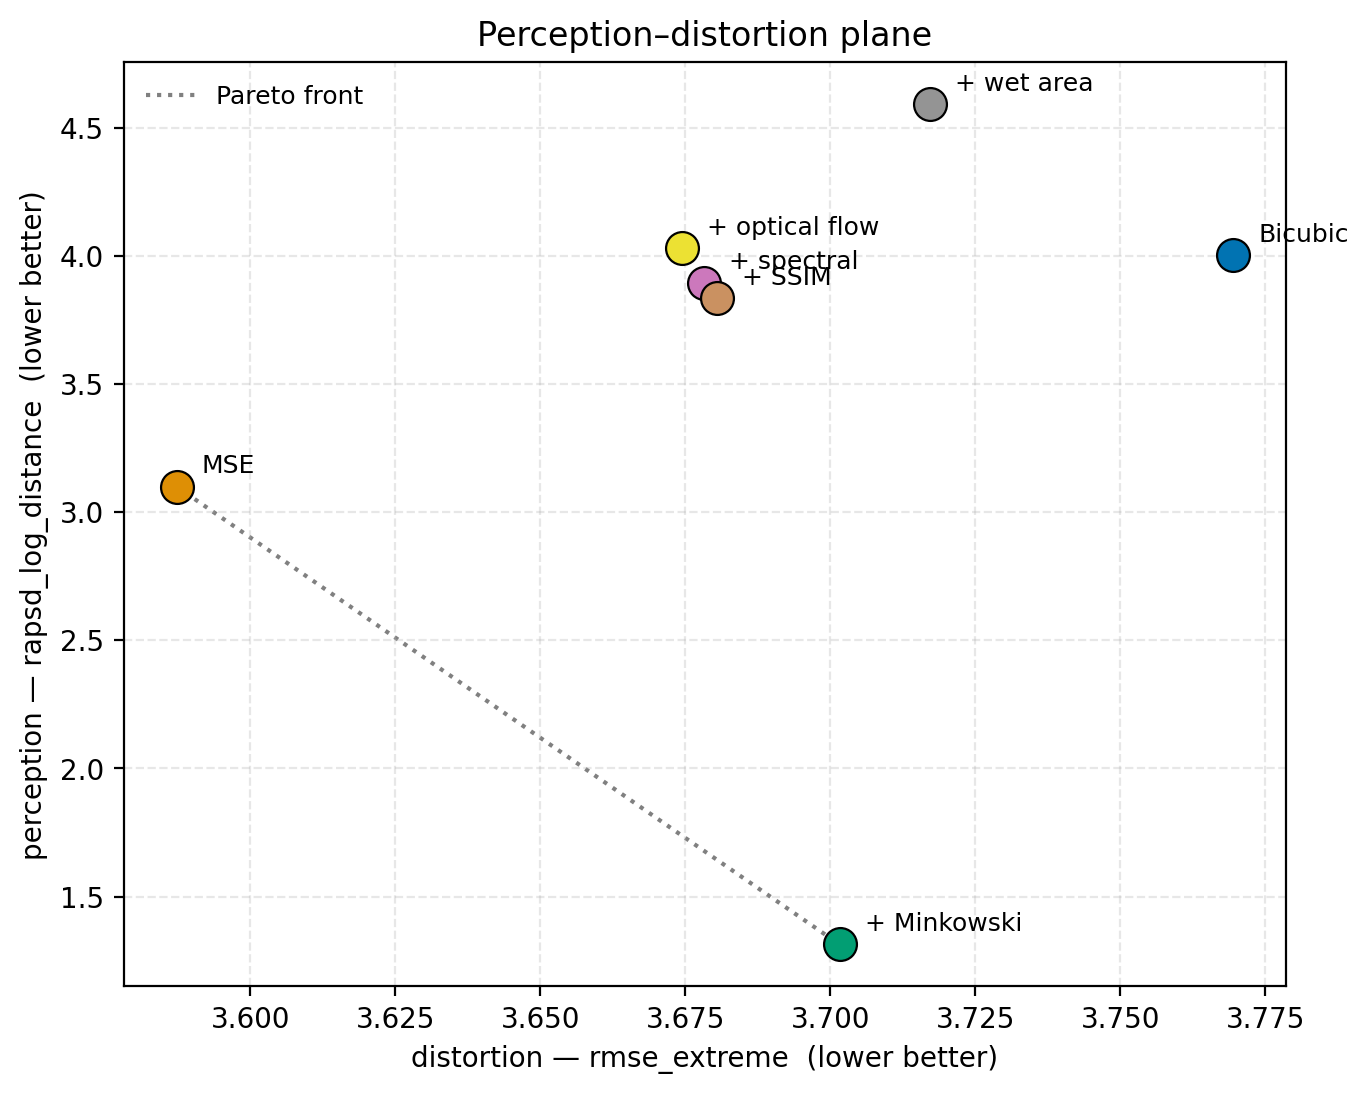
\includegraphics[width=0.49\textwidth]{study1/perception_distortion.png}
  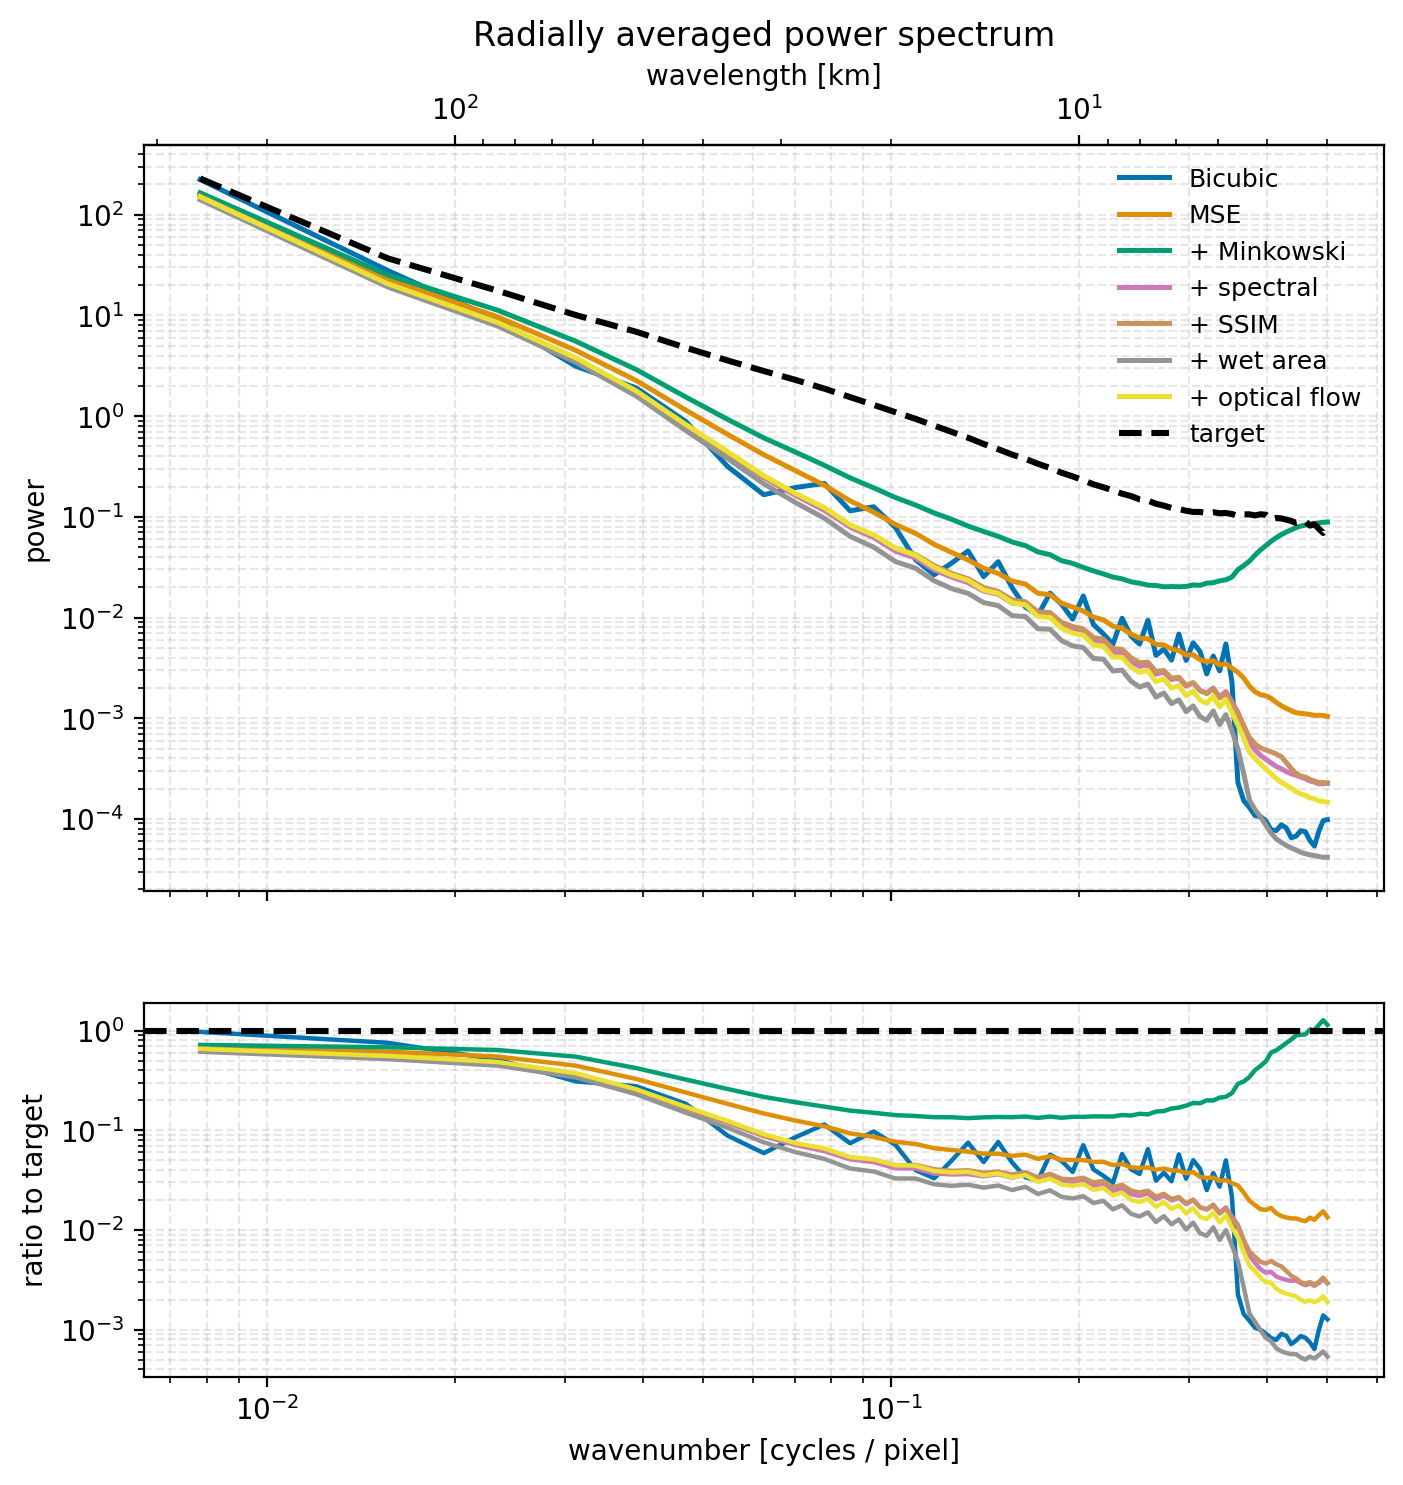
\includegraphics[width=0.49\textwidth]{study1/rapsd.png}
  \caption{Study~1. Left: the perception--distortion plane, extreme-conditioned root mean
  squared error against the spectral log-distance. The Pareto front contains two points, the
  mean-squared-error backbone and the Minkowski-trained backbone; all four competing losses
  are dominated, paying distortion without buying perception. Right: radially averaged power
  spectra with a predicted-to-target ratio panel. Every model tracks the target down to a
  wavelength of about $70\,\mathrm{km}$ and loses power below it, but by very different
  amounts: the worst-case power ratio is $\approx 0.12$ for the Minkowski-trained backbone,
  $\approx 0.04$ for mean squared error, and $0.02$--$0.03$ for the competing losses and
  bicubic interpolation.}
  \label{fig:study1}
\end{figure}

\begin{figure}[t]
  \centering
  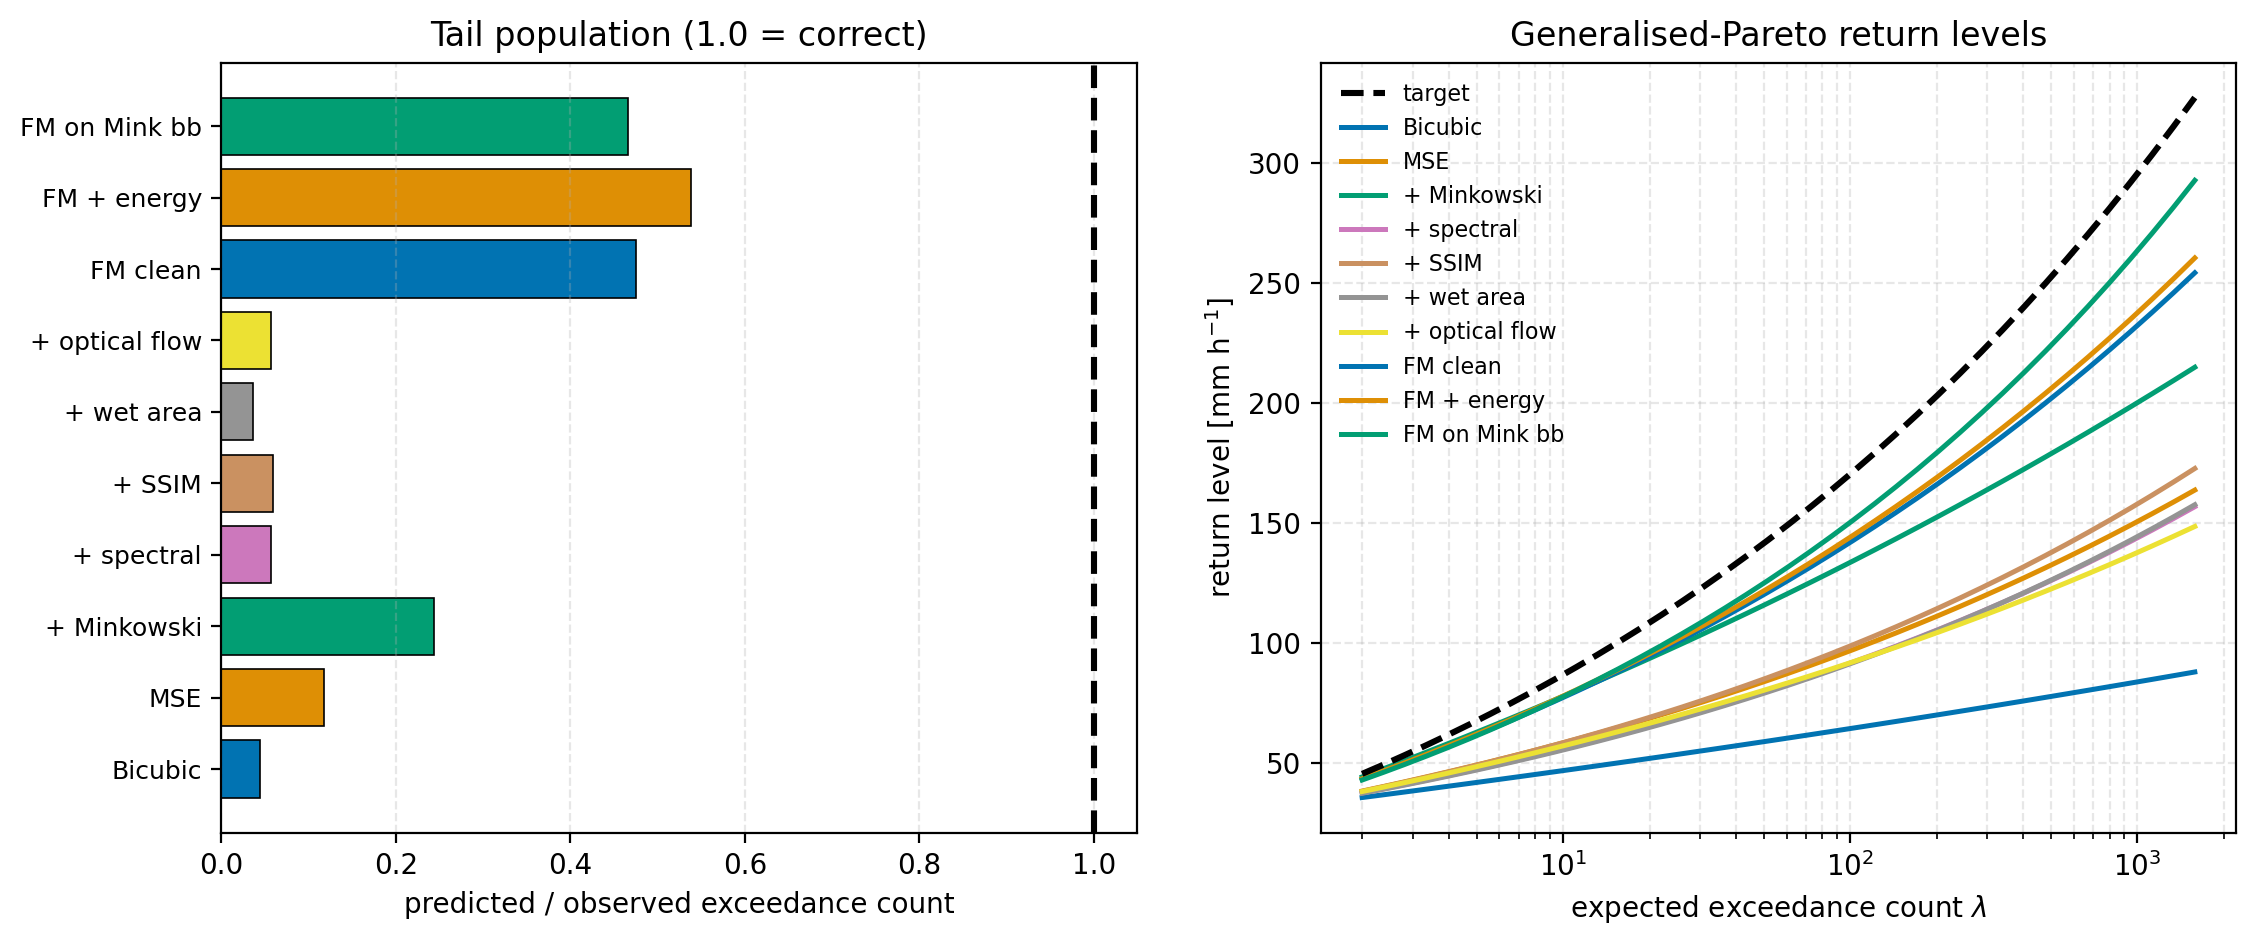
\includegraphics[width=0.49\textwidth]{all/tail_survival.png}
  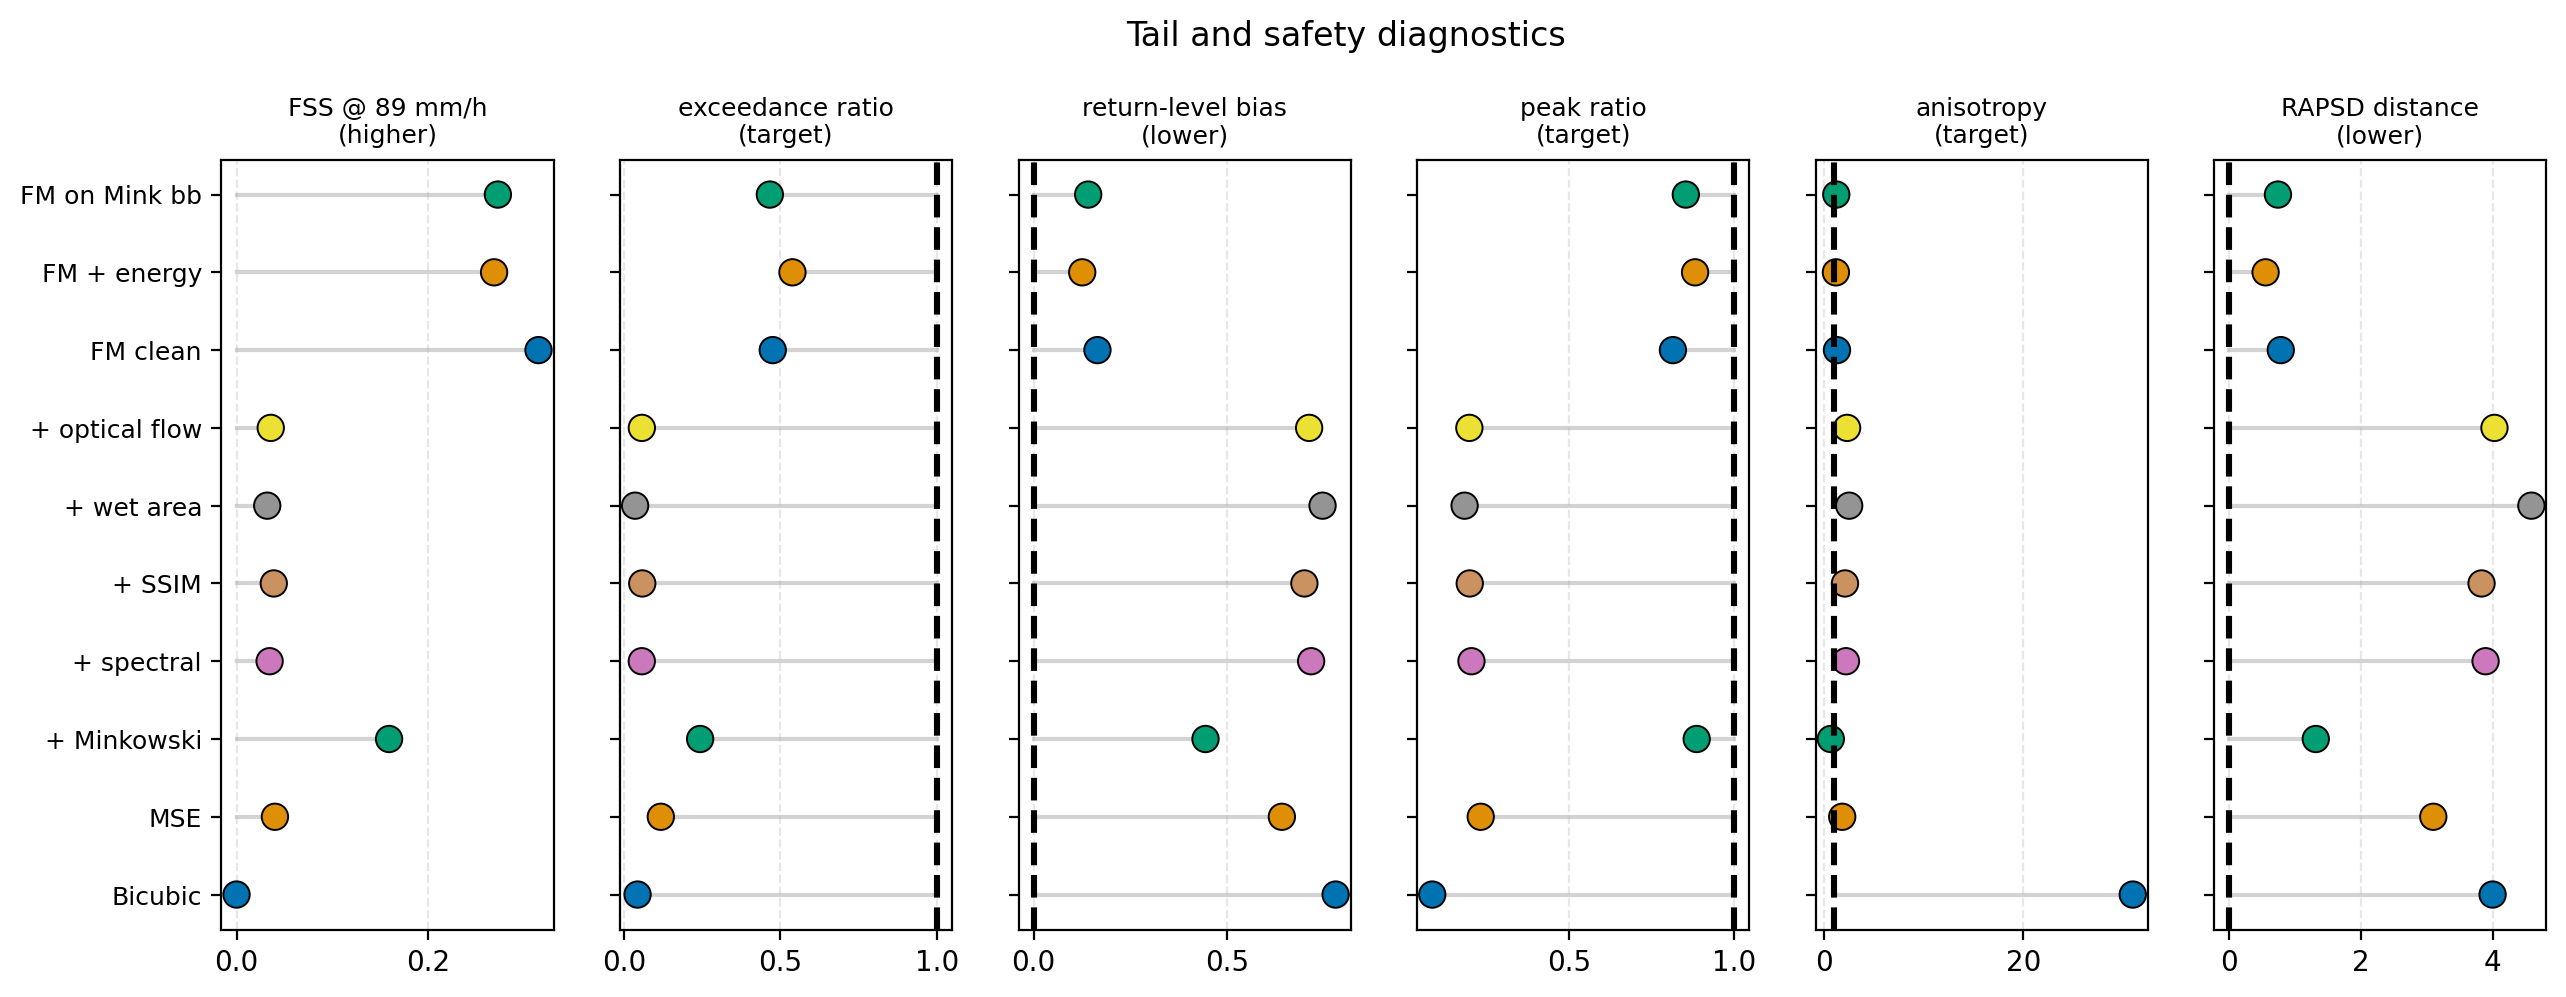
\includegraphics[width=0.49\textwidth]{all/tail_summary.png}
  % TODO: the label map in make_plots.py omits the per-sample reward cell (fm_reward) from
  % this figure; re-plot with it included before submission.
  \caption{Tail behaviour. Left: survival functions and generalised-Pareto return levels
  against expected exceedance count, fitted at $u = 31\,\mathrm{mm\,h^{-1}}$. Right: the tail
  and safety diagnostics of Table~\ref{tab:iid} on one axis -- exceedance ratio and peak ratio
  toward $1$, return-level bias toward $0$, directional anisotropy toward $1$. The anisotropy
  panel is dominated by bicubic interpolation at $30.9$; all trained models lie between $0.7$
  and $2.6$.}
  \label{fig:tails}
\end{figure}

\paragraph{Coupling the loss to the generative model.} The reward is correctly wired and its
effect is small. On a fixed-noise batch the reward falls by $59.7\,\%$ over fine-tuning, and
the truncated-back-propagation gradient is stable in the truncation depth: the cosine
similarity between the $K = 1$ and $K = 2$ gradients is $+0.91$, so $K = 1$ loses nothing and
the deeper, more expensive truncation is unnecessary.

With the coupling verified, the measured improvement is smaller than the spread of the
evaluation itself on most columns, and we report only what survives that comparison
(Table~\ref{tab:spread}). Two things do. The exceedance ratio rises from $0.475$ to $0.534$
with the per-sample reward and $0.538$ with the energy score, about three times the two-draw
movement of $0.021$; the spectral log-distance falls from $0.78$ to $0.65$ and $0.55$, about
one and a half times its movement of $0.084$. Both are tail-amplitude readouts of the same
change, and both cost less than $0.3\,\%$ in root mean squared error. Everything else we
might have claimed does not survive: the return-level bias, the peak ratio, the anisotropy
and the fractions skill score all move less between the clean and coupled models than they do
between two draws of the same model, so we do not read them, and in particular we cannot
separate the two reward forms on the fractions skill score, which is where the theory of
Section~\ref{sec:theory} predicts they should differ. That prediction -- that a
distributional reward constrains amplitude while leaving placement free -- remains untested
rather than confirmed.

Routing the loss in through the backbone instead of the reward is the weakest of the three
couplings, and here the evidence is only suggestive: a flow-matching model trained on the
Minkowski backbone has a lower exceedance ratio than the clean model ($0.466$ against
$0.475$), but that difference is half the two-draw movement. What can be said is the negative:
on no column does routing through the backbone improve on the clean model by more than the
evaluation moves by itself. The structural fidelity of the conditional mean does not visibly
propagate through the residual, which is the confound that motivated separating the two
studies in the first place; whether it does so weakly is below our current resolution.

\paragraph{Why the generative gain is small: a pixel-mass bottleneck.} A per-threshold
decomposition of the structural gradient on a batch containing a $142\,\mathrm{mm\,h^{-1}}$
patch explains the asymmetry. Thresholds at or below $0.28\,\mathrm{mm\,h^{-1}}$ carry
$83\,\%$ of the gradient; the $19\,\mathrm{mm\,h^{-1}}$ level carries $0.13\,\%$; levels at
and above $31\,\mathrm{mm\,h^{-1}}$ carry essentially none -- and it is precisely there that
the structural residual is largest ($0.8$--$1.2$ in log-$\gamma$ units, against near-zero in
the bulk). The cause is pixel mass rather than weighting: only about $5 \times 10^{-5}$ of
pixels exceed $31\,\mathrm{mm\,h^{-1}}$ and almost none exceed $53$, so the excursion sets
that define the extreme thresholds are empty in nearly every sample and contribute no
gradient at all. Re-weighting the threshold integral cannot manufacture a gradient from an
empty set. Neither can the indicator temperature: sweeping the anneal parameter from $0.05$
to $0.40$ raises the \emph{absolute} gradient at $31\,\mathrm{mm\,h^{-1}}$ by eleven orders of
magnitude, but the tail's \emph{share} of the total stays at $0.75$--$0.88\,\%$ and slightly
declines, because a wider indicator amplifies the bulk equally while degrading the bulk
excursion-set estimate. The remaining levers are therefore sample selection -- drawing the
structural batches from the patches that contain extremes -- and threshold reweighting
combined with it, not smoothing. This also explains why the loss helps the deterministic
backbone so much more: the backbone starts with a peak ratio of $0.23$, so even the
bulk-dominated gradient has a large, systematic error to correct, whereas the clean
generative model starts at $0.81$ and the remaining error lives almost entirely in the
threshold range where the gradient vanishes.

\paragraph{How large a difference is readable.} The flow-matching rows carry a sampling
uncertainty that we can measure rather than assume, because two of those cells were evaluated
twice. The two evaluations share the same $4{,}096$ patches: the observed exceedance count
($5{,}070$), the fitted observed shape and scale, and the observed return levels agree to
every recorded digit, so the target side is identical and only the generated ensembles differ.
Table~\ref{tab:spread} gives the resulting column-by-column movement between the two draws.

\begin{table}[t]
  \centering
  \small
  \caption{Movement of each column between two evaluations of the same checkpoints on the
  same $4{,}096$ patches, differing only in the ensemble draw, against the improvement each
  reward form shows over the clean model in Table~\ref{tab:iid}. A gain smaller than the
  two-draw movement is not readable. Two draws give a range, not a standard error; these are
  lower bounds on the spread.}
  \label{tab:spread}
  \resizebox{\textwidth}{!}{%
  \begin{tabular}{lccc}
    \toprule
    Column & two-draw movement & gain, per-sample reward & gain, energy score \\
    \midrule
    Exceedance ratio            & 0.021 & \textbf{0.059} & \textbf{0.063} \\
    RAPSD log-distance          & 0.084 & \textbf{0.131} & \textbf{0.231} \\
    Peak ratio (median)         & 0.025 & 0.021 & 0.067 \\
    Return-level bias           & 0.095 & 0.051 & 0.040 \\
    Anisotropy                  & 0.070 & 0.030 & 0.107 \\
    FSS at $89\,\mathrm{mm\,h^{-1}}$ & 0.124 & 0.006 & 0.046 \\
    RMSE on extremes            & 0.013 & 0.002 & 0.011 \\
    \bottomrule
  \end{tabular}}
\end{table}

Two consequences follow, and they are restrictive. The fractions skill score moves by up to
$0.124$ between draws -- as much as the entire spread across the four flow-matching cells --
so no difference within that block is readable from it, including the apparent separation
between the two reward forms. The return-level bias moves by up to $0.095$, which is larger
than the coupling's apparent gain of $0.051$; it is an extrapolation from a fitted tail to
$\lambda = 10^3$ and therefore amplifies fit noise, whereas the exceedance ratio is a direct
count and moves by only $0.021$. Of the columns in Table~\ref{tab:iid}, only the exceedance
ratio and the spectral log-distance show a coupling gain that exceeds the two-draw movement,
by factors of about three and one and a half.

We cannot yet separate two explanations for that movement. The ensemble draw is not seeded, so
it may be ordinary Monte Carlo variance of $M = 16$ samples; alternatively the earlier
evaluation may have used a different checkpoint of the same run, since the summaries do not
record which checkpoint was evaluated. The two are distinguished by one cheap experiment --
evaluate one cell three times from the same checkpoint with different sampling seeds -- and
that experiment, not a larger patch subset, is what these rows need before any of them is
quoted as a finding. We report the numbers with the movement attached rather than omitting
either.

The deterministic block does not have this problem: it is a deterministic forward pass over
$285{,}383$ patches with $316{,}652$ exceedances, so repeated evaluation is exact, and the
Minkowski-versus-baseline gaps there are between two and four times the spread across the four
competing losses. All rows remain single-seed with respect to \emph{training}, which is a
separate and larger uncertainty that we have not quantified for any model.

\begin{table}[t]
  \centering
  \small
  \setlength{\tabcolsep}{4pt}
  \caption{Out-of-distribution extremes. Placeholder -- same columns and same
  peaks-over-threshold level as Table~\ref{tab:iid}, on held-out out-of-distribution events.
  Not yet run.}
  \label{tab:ood}
  \resizebox{\textwidth}{!}{%
  \begin{tabular}{lcccccccc}
    \toprule
    Model & RMSE$_{\mathrm{ext}}\downarrow$ & FSS$\uparrow$ &
    RAPSD$\downarrow$ & Mink.$\downarrow$ & Exc.$\to 1$ &
    RL bias$\downarrow$ & Peak $\to 1$ & Anis.$\to 1$ \\
    \midrule
    Bicubic                     & -- & -- & -- & -- & -- & -- & -- & -- \\
    MSE backbone                & -- & -- & -- & -- & -- & -- & -- & -- \\
    \quad + Minkowski           & -- & -- & -- & -- & -- & -- & -- & -- \\
    Flow matching (clean)       & -- & -- & -- & -- & -- & -- & -- & -- \\
    \quad + Minkowski reward    & -- & -- & -- & -- & -- & -- & -- & -- \\
    \bottomrule
  \end{tabular}}
\end{table}

\section{Discussion}
% ---------------------------------------------------------------------
\label{sec:disc}
The two studies answer their research questions asymmetrically, and the asymmetry is the
result worth carrying forward.

For the deterministic backbone (research question~2) the answer is affirmative and large.
The mean-squared-error backbone fails in the predicted way -- structure, not amplitude or
location, is the deficient SAL component -- and the Minkowski image loss removes most of that
deficit while doubling the reproduced tail mass and cutting the return-level bias by a third,
for under four percent of point accuracy. None of the four competing structural losses does
anything comparable at a weight that leaves point accuracy intact. The distinguishing feature
of the Minkowski loss in this comparison is that it constrains excursion sets at prescribed
intensities, so the quantity it protects is the one that pixelwise training destroys: the
baseline retains $23\,\%$ of the median patch maximum, the Minkowski-trained model $89\,\%$.
The spectral and structural-similarity losses constrain second-order or perceptual statistics
that a smoothed field can satisfy without carrying any peak at all.

For the generative stage (research question~1) the answer is at the resolution limit of our
evaluation, and the reason the effect is small is mechanical rather than a failure of the
coupling. The coupling is verifiably wired:
the reward falls by $60\,\%$ on a fixed-noise batch and the truncated gradient is stable in
its depth. What limits it is pixel mass. Above $31\,\mathrm{mm\,h^{-1}}$ the excursion sets
are empty in nearly every sample, so $83\,\%$ of the structural gradient comes from drizzle
thresholds, and neither threshold reweighting nor indicator smoothing can change that -- the
anneal sweep moves the tail gradient by eleven orders of magnitude in absolute terms and
leaves its share of the total unchanged. The deterministic backbone gains so much more
because it begins with a large, systematic error that even a bulk-dominated gradient can
correct; the clean flow-matching model begins close enough that the residual error lives
where the gradient does not. This identifies the next experiment precisely: select the
structural batches from the patches that contain extremes, keeping the mean-squared-error and
velocity terms on uniformly drawn batches so the conditional mean remains
$\mathbb{E}[y \mid c]$.

The $10^{-3}$ episode is a result in its own right rather than a failed run. A model that
improves every structural metric in the protocol while inventing grid-aligned filaments is a
concrete instance of the theoretical limit of Section~\ref{sec:theory}: Hadwiger completeness
concerns the basis of valuations, not identifiability of the field law, so matching Minkowski
curves is necessary and not sufficient. The practical consequence is that a structural-loss
protocol needs at least one diagnostic that no loss in the comparison optimises. Directional
anisotropy and the peak ratio serve that role here, and the bicubic baseline's anisotropy of
$30.9$ against the models' $0.7$--$2.6$ shows the diagnostic has the dynamic range to detect
the pathology it was added for.

Three questions remain open. Whether $\chi$ is the wrong topological target for hole-rich
precipitation fields, with $\beta_0$ the better one, is settled by a confirmatory run at the
winning weight in the persistent-homology mode, which we have not run; the mathematical
expectation -- $\chi = \beta_0 - \beta_1$ being $\beta_1$-dominated -- gives the hypothesis,
not the answer. Whether the competing losses are genuinely weaker or merely under-weighted
requires re-running them at a weight that costs several percent of mean absolute error, and
we report the weaker conclusion until that is done. Finally, the out-of-distribution
protocol (Table~\ref{tab:ood}) is the test that matters most for the claim in the title, and
it is not yet run: every number above is in-distribution, and a structural loss that improves
in-distribution tail statistics may or may not transfer to events outside the training
distribution.

% =====================================================================
\section{Conclusion}
% ---------------------------------------------------------------------
% [Draft -- revisit once the o.o.d. protocol and the beta_0 confirmatory run are done.]
The Minkowski image loss improves the extreme tail of a deterministic precipitation
downscaler substantially and at a small, quantified accuracy cost: on $12.5\times$
super-resolution of OPERA radar, it doubles the reproduced exceedance mass above
$31\,\mathrm{mm\,h^{-1}}$, cuts the mean absolute return-level bias by a third, quadruples the
fractions skill score at $89\,\mathrm{mm\,h^{-1}}$, and raises the median retained patch
maximum from $0.23$ to $0.89$, for $+3.8\,\%$ mean absolute error. Four competing structural
losses achieve none of this at weights that leave point accuracy intact. Coupling the same
loss to a residual flow-matching model through truncated back-propagation of the
probability-flow solver improves the tail far less, and on most columns by less than the
evaluation moves between two draws of the same ensemble; only the exceedance ratio and the
spectral log-distance show a gain larger than that movement. We attribute the small size of
the effect to a measured pixel-mass bottleneck rather than to the coupling: above
$31\,\mathrm{mm\,h^{-1}}$ the excursion sets are empty in almost every sample, so the
structural gradient is dominated by drizzle thresholds regardless of how the threshold
integral is weighted or how wide the soft indicator is made. The implication for structural
losses in general is that their reach into the tail is set by how often the tail is populated
in a training batch, which makes sample selection, not loss design, the next lever. We also
report a negative result with a positive use: at a ten-fold larger weight the loss is
straightforwardly hacked -- every structural metric improves while the model invents
grid-aligned filaments -- which makes concrete the gap between matching a complete basis of
valuations and identifying the field law, and argues that any structural-loss protocol should
carry a diagnostic that none of its losses optimises. The out-of-distribution evaluation, a
confirmatory run in the $\beta_0$ topology mode, and a replication across seeds remain to be
done, as does generalisation beyond radar to model output such as COSMO.

\bibliographystyle{unsrtnat}
\bibliography{references}

\end{document}